\hypertarget{ht__init_8c}{
\section{ht\_\-init.c File Reference}
\label{ht__init_8c}\index{ht_init.c@{ht\_\-init.c}}
}


\subsection{Detailed Description}
\begin{Desc}
\item[For internal use only.]
This file contains the implementation of the \hyperlink{group__dbprim__hash_ga10}{ht\_\-init()} function, used to dynamically initialize a hash table.\end{Desc}


Definition in file \hyperlink{ht__init_8c-source}{ht\_\-init.c}.

{\tt \#include $<$errno.h$>$}\par
{\tt \#include $<$stdlib.h$>$}\par
{\tt \#include \char`\"{}dbprim.h\char`\"{}}\par
{\tt \#include \char`\"{}dbprim\_\-int.h\char`\"{}}\par


Include dependency graph for ht\_\-init.c:\begin{figure}[H]
\begin{center}
\leavevmode
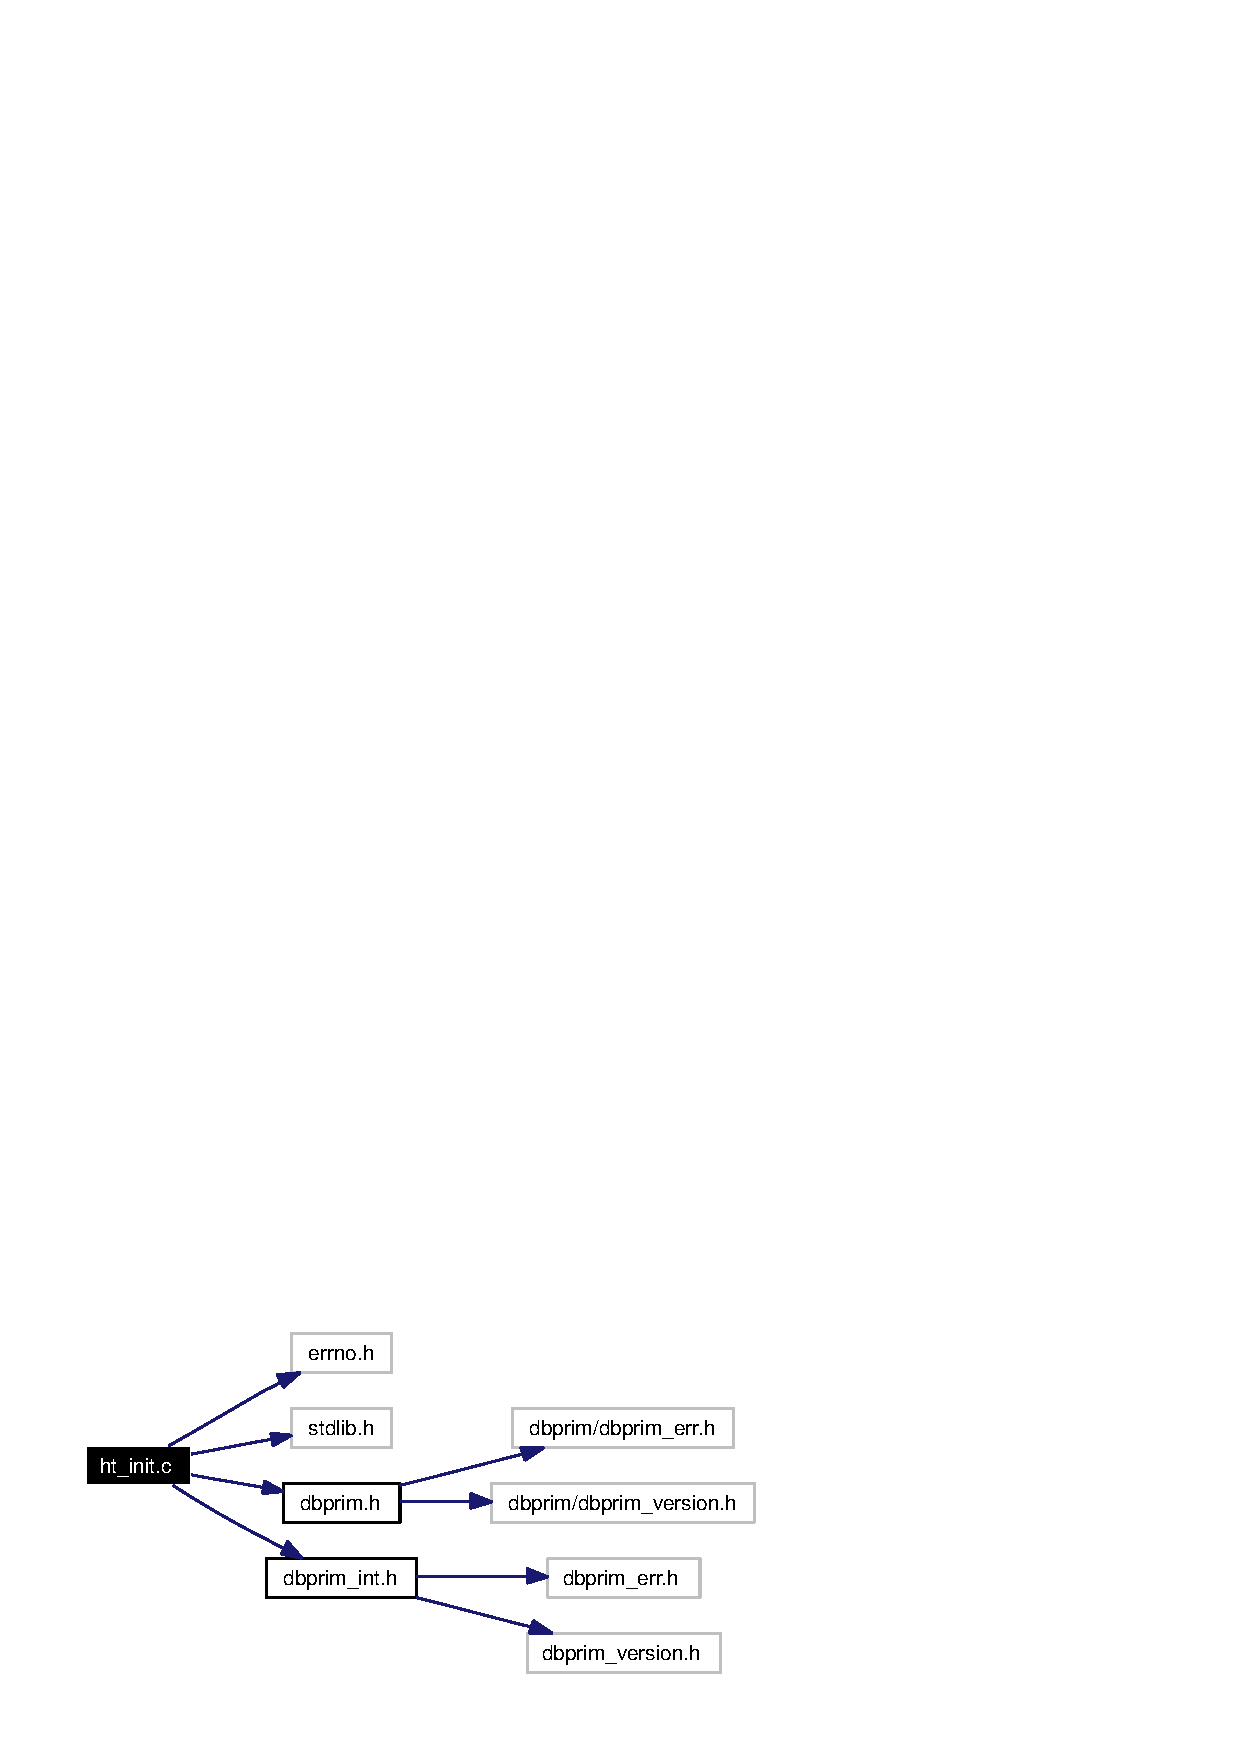
\includegraphics[width=183pt]{ht__init_8c__incl}
\end{center}
\end{figure}
\subsection*{Functions}
\begin{CompactItemize}
\item 
unsigned long \hyperlink{group__dbprim__hash_ga10}{ht\_\-init} (\hyperlink{struct__hash__table__s}{hash\_\-table\_\-t} $\ast$table, unsigned long flags, \hyperlink{group__dbprim__hash_ga4}{hash\_\-func\_\-t} func, \hyperlink{group__dbprim__hash_ga5}{hash\_\-comp\_\-t} comp, \hyperlink{group__dbprim__hash_ga6}{hash\_\-resize\_\-t} resize, void $\ast$extra, unsigned long init\_\-mod)
\begin{CompactList}\small\item\em Dynamically initialize a hash table. \item\end{CompactList}\end{CompactItemize}
